\documentclass[10pt, oneside]{article}   	
\usepackage[left=20mm,top=20mm,right=20mm,bottom=20mm]{geometry}   
\geometry{a4paper}
\usepackage{algorithm,algpseudocode}  
\usepackage{graphicx}					
\usepackage{amssymb}
\usepackage{amsmath}
\usepackage{gensymb}
\usepackage{url}
\usepackage{titlesec}
\usepackage[parfill]{parskip}
\usepackage{cite}
\usepackage{array}
\usepackage{siunitx}
\usepackage{listings}
\usepackage{fixltx2e}
\usepackage{color}
\usepackage[usenames,dvipsnames,svgnames,table]{xcolor}
\usepackage[parfill]{parskip}
\setlength{\headsep}{5pt}
\graphicspath{ {images/} }
\lstset{
  basicstyle=\ttfamily,
  columns=fixed,
  fontadjust=true,
  basewidth=0.5em
}
\titleformat{\section}
{\normalfont\large\bfseries}{\thesection}{1em}{}
\titleformat{\subsection}
{\normalfont\normalsize\bfseries}{\thesubsection}{1em}{}
\title{\vspace{-1.6cm}INCA Open Examination Report}
\author{Exam Number: Y3603***}
\date{}							
\begin{document}
\maketitle
\section{Discussion of architectures} \label{sec:architectures}
The type of problem required to be solved with a neural network is a classification problem -- that is, to decide class membership of an unknown data item, based on another data set of data items with known class memberships \cite[Sec. 2]{Dreiseitl2002352}. Depending on the target output, the purpose could be to classify a set of inputs into two or more classes. This problem requires the simplest form of binary classification \cite[Fig. 4]{candanedo2016accurate}, where the output should be either \textit{yes} (room occupied) or \textit{no} (unoccupied). 

Given the nature of the problem, a wide range of feedforward architectures can be chosen. This section gives a brief discussion on the features of each architecture, and performs test-runs of that architecture's network in various configurations to find the best cursory performance. The MATLAB Neural Network Toolbox \cite{kohonen2014matlab} will be used throughout this report, unless otherwise noted.

The data used in these cursory test-runs are directly imported from the data CSVs with minimal processing. The training dataset is used to train the networks, while the two test datasets merged into one (for now) is used to test the networks on unseen data. Input and target datasets are separated due to toolbox requirements. At this stage, the only pre-processing done is the removal of time, which will be later experimented with the chosen architecture.

\subsection{Multilayer perceptron networks with backpropagation}

Multilayer perceptron (MLP) is a typical feedforward neural network. In a MLP, neurons are arranged in layers, which consist of an input layer, one or more hidden layers, and an output layer. The feedforward property means that neurons are connected from one layer to the next with no `lateral' or `feedback' connections \cite{som-lecture}, and the backpropagation property through training functions implies the network's ability to propagate errors at the output layer back through the network to update weights during training, improving performance. MLP requires supervised training -- with known target for the training dataset. MLP is useful to solve both regression and classification problems, but careful control of network configuration and training parameters is required to avoid overfitting. The selection of number of layers and layer sizes are important in creating accurate and useful MLP networks.

Three different backpropagation training functions are used for MLP: Levenberg-Marquardt ($trainlm$), gradient descent ($traingd$), and gradient descent with momentum ($traingdm$) for updating weight and bias values during training. All three are trained on the training dataset with various layer configurations to test for best performance. The performance here is measured by two indices: the mean square error (MSE) and the actual misclassification rate (with classification determined by rounding to 0 or 1), both on the testing dataset unseen during training, as in practical use the network nearly always works with unseen data. All other parameters are toolbox default. The results of the testing can be seen in Figure \ref{fig:mlp-testing}.

\begin{figure}[h]
\begin{center}
\fontsize{9}{11}\selectfont
\begin{tabular}{|c|c|c|c|c|c|}
\hline 
MLP Configuration & [5 3 2] & [6 4 2] & [10 5 5] & [20 10 10] & [6 4] \\ \hline \hline 
$trainlm$ Validation MSE & 0.077 & 0.090 & 0.062 & 0.093 & 0.045 \\ \hline 
$trainlm$ Misclassification (\%) & 7.87 & 9.63 & 6.21 & 9.87 & 8.15 \\ \hline \hline 
$traingd$ Validation MSE & 0.149 & 0.053 & 0.101 & 0.054 & 0.088 \\ \hline 
$traingd$ Misclassification (\%) & 16.5 & 4.16 & 10.2 & 6.19 & 11.8 \\ \hline \hline 
$traingdm$ Validation MSE & 0.046 & 0.197 & 0.109 & 0.033 & 0.032 \\ \hline 
$traingdm$ Misclassification (\%) & 5.87 & 27.5 & 16.9 & 2.24 & 3.31 \\ \hline 
\end{tabular}
\end{center}
\caption{\label{fig:mlp-testing} Results from cursory testing of multilayer perceptron (MLP) networks.}
\end{figure}

Barring the large [20 10 10] architecture (while the best external validation performance for $traingdm$, is slow to train and has a tendency to overfit other training data), the best performing architectures for $trainlm$, $traingd$ and $traingdm$ appear to be [10 5 5], [6 4 2] and [6 4] respectively. It is worth nothing that these are performed on data with limited preprocessing, and are indicative only to determine what configurations or similar configurations could be potentially used if MLP is chosen to be the final architecture.

\subsection{Radial basis function networks}

The radial basis function (RBF) network is another feedforward architecture with the ability to solve linearly inseparable classification problems. Rather than using hidden layers of identical neurons to achieve this like MLP, a RBF network transforms data into a higher dimension through the use of a layer of fully connected neurons computing radial basis functions \cite{rbf-lecture}. This often allows the RBF network to solve classification problems more efficiently than MLP, but at the same time makes training on large data samples a slow process, due to the need of computing large numbers of distinct basis functions \cite[p. 260]{haykin2008}.

The toolbox provides two methods for creating an RBF network: exact fit and fewer neurons. The former, while fast, is not used due to its high tendency of overfitting. The latter requires a definite goal MSE as stopping condition, thus requires much more time to train, but does not have the disadvantage of the exact fit method. Based on the MSEs seen during MLP training, four goals are used to train four different RBF networks, as shown in Figure \ref{fig:rbf-testing}. All other parameters are toolbox defaults.

\begin{figure}[h]
\begin{center}
\fontsize{9}{11}\selectfont
\begin{tabular}{|c|c|c|c|c|c|}
\hline 
RBF Training MSE Goal & 0.2 & 0.1 & 0.05 & 0.01 & 0.001 \\ \hline \hline 
Validation MSE & 0.185 & 0.197 & 0.214 & 0.234 & 0.240 \\ \hline 
Misclassification (\%) & 24.33 & 24.31 & 24.31 & 24.28 & 24.27 \\ \hline 
\end{tabular}
\end{center}
\caption{\label{fig:rbf-testing} Results from cursory testing of radial basis function (RBF) networks.}
\end{figure}

From past experience with the toolbox, training of RBF networks with the toolbox appears to be deterministic. It can be observed that RBF networks perform significantly worse than MLP networks (Figure \ref{fig:mlp-testing}) with the same input, especially in terms of actual misclassification rate on unseen data.

\subsection{Self-organising maps} \label{subsec:som-test}

Self-organising maps (SOM) is a feedforward neural network architecture often used for specialised purposes such as data visualisation. The network consists of a mesh of connected neurons that attempts to rearrange positions match a data distribution in a iterative process \cite[p. 34]{som-lecture}. While it is often used to reduce the dimension of data for visualisation purposes, it can also be used to solve classification problems \cite{owens2000application}. 

In particular, SOM is able to produce a out-dimensional output mesh from a multi-dimensional input dataset, allowing the computation of both linear regression and classification problems, as demonstrated by Haykin \cite[Sec. 9.5]{haykin2008}. This allows the binary classification problem to be solved by fitting a one-dimensional mesh to the training data, and determining which side of the mesh is a testing input placed. Further more, SOM deploys unsupervised learning and does not require targets for training data. This reduces the likelihood of bias towards patterns of training data, and allows continuous training in use.

The same training and testing datasets as used for MLP and RBF networks are used to evaluate SOM performance, with varying single-dimensional mesh sizes (also the number of neurons), as shown in Figure \ref{fig:som-testing}. Toolbox defaults such as $hexgrid$ and $linkdist$ are used.

\begin{figure}[h]
\begin{center}
\fontsize{9}{11}\selectfont
\begin{tabular}{|c|c|c|c|c|c|c|}
\hline 
SOM Mesh Size & [2 1] & [5 1] & [10 1] & [20 1] & [30 1] & [40 1] \\ \hline 
Validation MSE & 0.113 & 0.090 & 0.055 & 0.084 & 0.138 & 0.125 \\ \hline 
Misclassification (\%) & 24.3 & 11.3 & 7.33 & 3.21 & 4.83 & 3.74 \\ \hline \hline 
SOM Mesh Size & [50 1] & [60 1] & [70 1] & [80 1] & [90 1] & [100 1] \\ \hline 
Validation MSE & 0.162 & 0.138 & 0.150 & 0.166 & 0.207 & 0.225 \\ \hline 
Misclassification (\%) & 11.1 & 10.8 & 9.89 & 11.7 & 30.2 & 29.7 \\ \hline 
\end{tabular}
\end{center}
\caption{\label{fig:som-testing} Results from cursory testing of self-organising maps (SOM).}
\end{figure}

It can be observed that SOM exhibits a steady and accurate performance between 10 and 40 neurons in the mesh. The best performance with 20 neurons is comparable to those of MLP.

\subsection{Selection of the final architecture}

Based on the results from cursory testings of the three architectures discussed, as well their characteristics, the \textbf{self-organising map (SOM)} is chosen as the final architecture for further experimentation. 

RBF is firstly ruled out due to its consistently high misclassification rate observed on unseen data, making it undesirable for the purpose of the problem: accurately identify the occupancy of a room based on sensor data only. While different MLP training functions do produce comparable performance to SOM at different layer configurations, it is ultimately decided that the constant influx of new data during the operation of the occupancy identification system would create hassle in constantly sourcing data for the supervised training of MLP, as the patterns in sensor data will change as the season or other environmental conditions change. The unsupervised training of SOM allows the system to take into account new data in far less computational expensive way. Thus, MLP is also ruled out, leaving SOM as the chosen architecture.

In addition, a few more runs of the cursory testing also shows that the misclassification rates of MLP fluctuate more significantly than SOM, which could potentially cause the system to be less stable in producing accurate results if MLP is used in place of SOM. 

\section{Room occupancy detection with self-organising maps}

\subsection{Data exploration and pre-processing} \label{subsec:preprocessing}
While Section \ref{sec:architectures} merged the two testing datasets for convenience, according to the source of the data, the two testing datasets are different in nature: the much smaller first dataset was recorded mostly when the door to the room is closed, and the bigger second dataset was recorded mostly with the door open \cite[Tb. 5]{candanedo2016accurate}. Therefore, for the in-depth study of the data in this section, the two testing datasets will be processed separately. The number of inputs in the training dataset and the two test datasets (Validation 1, Validation 2) are 8143, 2665 and 9752 respectively.

Based on observations of results from $plotsomhits$ in cursory testing, an assumption is made that the SOM will always class the data on either end of the one-dimensional network, which has always been the case in the observed results. This is used to calculate the misclassification rate, based on which end is closer to the location the data is placed by the SOM. When high misclassification rates are observed after preprocessing procedures later in this section, $plotsomhits$ will be consulted again to ensure that the problem is not from this assumption. It is worth noting that the toolbox's SOM performs no preprocessing by default.

The training dataset will be used to train the SOM, while the two testing datasets will be used as unseen inputs to evaluate the performance of the trained SOM. There is no missing value. With the exception of time, all values are numerical. Therefore no imputation or numerical encodings are required. All three datasets exhibit a relative imbalance in class membership: the percentages of room unoccupied are 79\%, 64\% and 79\% respectively. While is could potentially cause a bias in training and testing data, it was decided that no rebalancing measures should be conducted, as (1) the training and testing datasets exhibit a common pattern, and (2) this appears to be the normal usage pattern of the room in question, as well as the fact that 79\% is not an overwhelming majority that could skew results, such as those observed in using SOM to detect transaction fraud (negative $>$99\%) \cite{almendra2014using}, which would require special measures for the SOM to function reliably. 

To further illustrate the effects of rebalancing, a comparison test was conducted with toolbox defaults between a training dataset of 1729 randomly sampled unoccupied inputs and all 1729 occupied inputs, and a training dataset of 3458 randomly sampled inputs with no particular pattern. Each side of comparison was freshly trained ten times, and the results are as shown in Figure \ref{fig:equalize-testing}, demonstrating that it is better \textit{not} to rebalance the inputs in SOM training. It is worth noting that as SOM deploys unsupervised training, the network is not aware of the class distribution of the training dataset.

\begin{figure}[h]
\begin{center}
\fontsize{9}{11}\selectfont
\begin{tabular}{|c|c|c|}
\hline 
Rebalance of Input Dataset & Rebalanced (1729 Positive + 1729 Negative) & Not Rebalanced (3458 Random) \\ \hline
Mean Training MSE & 0.096 & 0.055 \\ \hline \hline 
Mean Validation 1 MSE & 0.071 & 0.069 \\ \hline 
Mean Misclassification 1 (\%) & 8.96 & 2.18 \\ \hline \hline 
Mean Validation 2 MSE & 0.112 & 0.140 \\ \hline 
Mean Misclassification 2 (\%) & 16.08 & 9.23 \\ \hline
\end{tabular}
\end{center}
\caption{\label{fig:equalize-testing} Results from testing the balancing of training input on a [20 1] SOM. (All MSE variances $<0.01$, all \% variances $<2.00$.)}
\end{figure}

Two types of data based on time are provided: the sequence number and the exact time. Both of which could be potentially useful for the network, especially in studying the time-based occupation pattern of the room studied. But at the same time, this could cause the loss of generalisability, as well as affecting the network performance. In order to determine the suitability of using time, the best SOM configuration Section \ref{subsec:som-test} -- [20 1] is trained by three variations of the training dataset: time removed, with time sequence numbers, and with exact times converted into integer timestamps. In the latter two variations, the time variable is scaled to between 0 and 1. For all variations, the other five input variables are attached as is. The results of the testing can be found in Figure \ref{fig:time-testing}.

\begin{figure}[h]
\begin{center}
\fontsize{9}{11}\selectfont
\begin{tabular}{|c|c|c|c|}
\hline 
Time Variation in Input & No Time & Integer Timestamps & Time Sequence Numbers \\ \hline \hline 
Validation 1 MSE & 0.063 & 0.063 & 0.062 \\ \hline 
Misclassification 1 (\%) & 2.18 & 2.18 & 2.18 \\ \hline \hline 
Validation 2 MSE &  0.090 & 0.089 & 0.090 \\ \hline 
Misclassification 2 (\%) & 3.51 & 3.41 & 3.48 \\ \hline 
\end{tabular}
\end{center}
\caption{\label{fig:time-testing} Results from testing the use of time in training input on a [20 1] SOM.}
\end{figure}

From the results, it can be seen that the inclusion of time (in either form) has almost no effect on the performance of network on unseen test data, confirming the assessment specification that the other input variables (from sensor data) have already included the influence of time. Therefore, for the consideration of generalisability, time is removed from the input variables.

This leaves five input variables, all based on sensor data, as shown in Figure \ref{fig:final-variables}. 

\begin{figure}[h]
\begin{center}
\fontsize{9}{11}\selectfont
\begin{tabular}{|c|c|c|c|}
\hline 
\# & Input Variable & Type & Range \\ \hline 
1 & Temperature & Numeric & [19, 24.4083] \\ \hline 
2 & Humidity & Numeric & [16.745, 39.5] \\ \hline 
3 & Light & Numeric & [0, 1697.2] \\ \hline 
4 & CO\textsubscript{2} & Numeric & [412.75, 2076.5] \\ \hline
5 & Humidity Ratio & Numeric & [0.0027, 0.0065] \\ \hline
\end{tabular}
\end{center}
\caption{\label{fig:final-variables} Input variables to the SOM.}
\end{figure}

With five numeric input variables, two different forms of further pre-processing are possible: [0, 1] normalisation or principle component analysis (PCA) after variance standardisation. In order to better understand the characteristics of the input data, $plotmatrix$ is first performed on input variables in Figure \ref{fig:final-variables}, as shown on the left side of Figure \ref{fig:pca-before-after}.

\begin{figure}[h]
\begin{center}
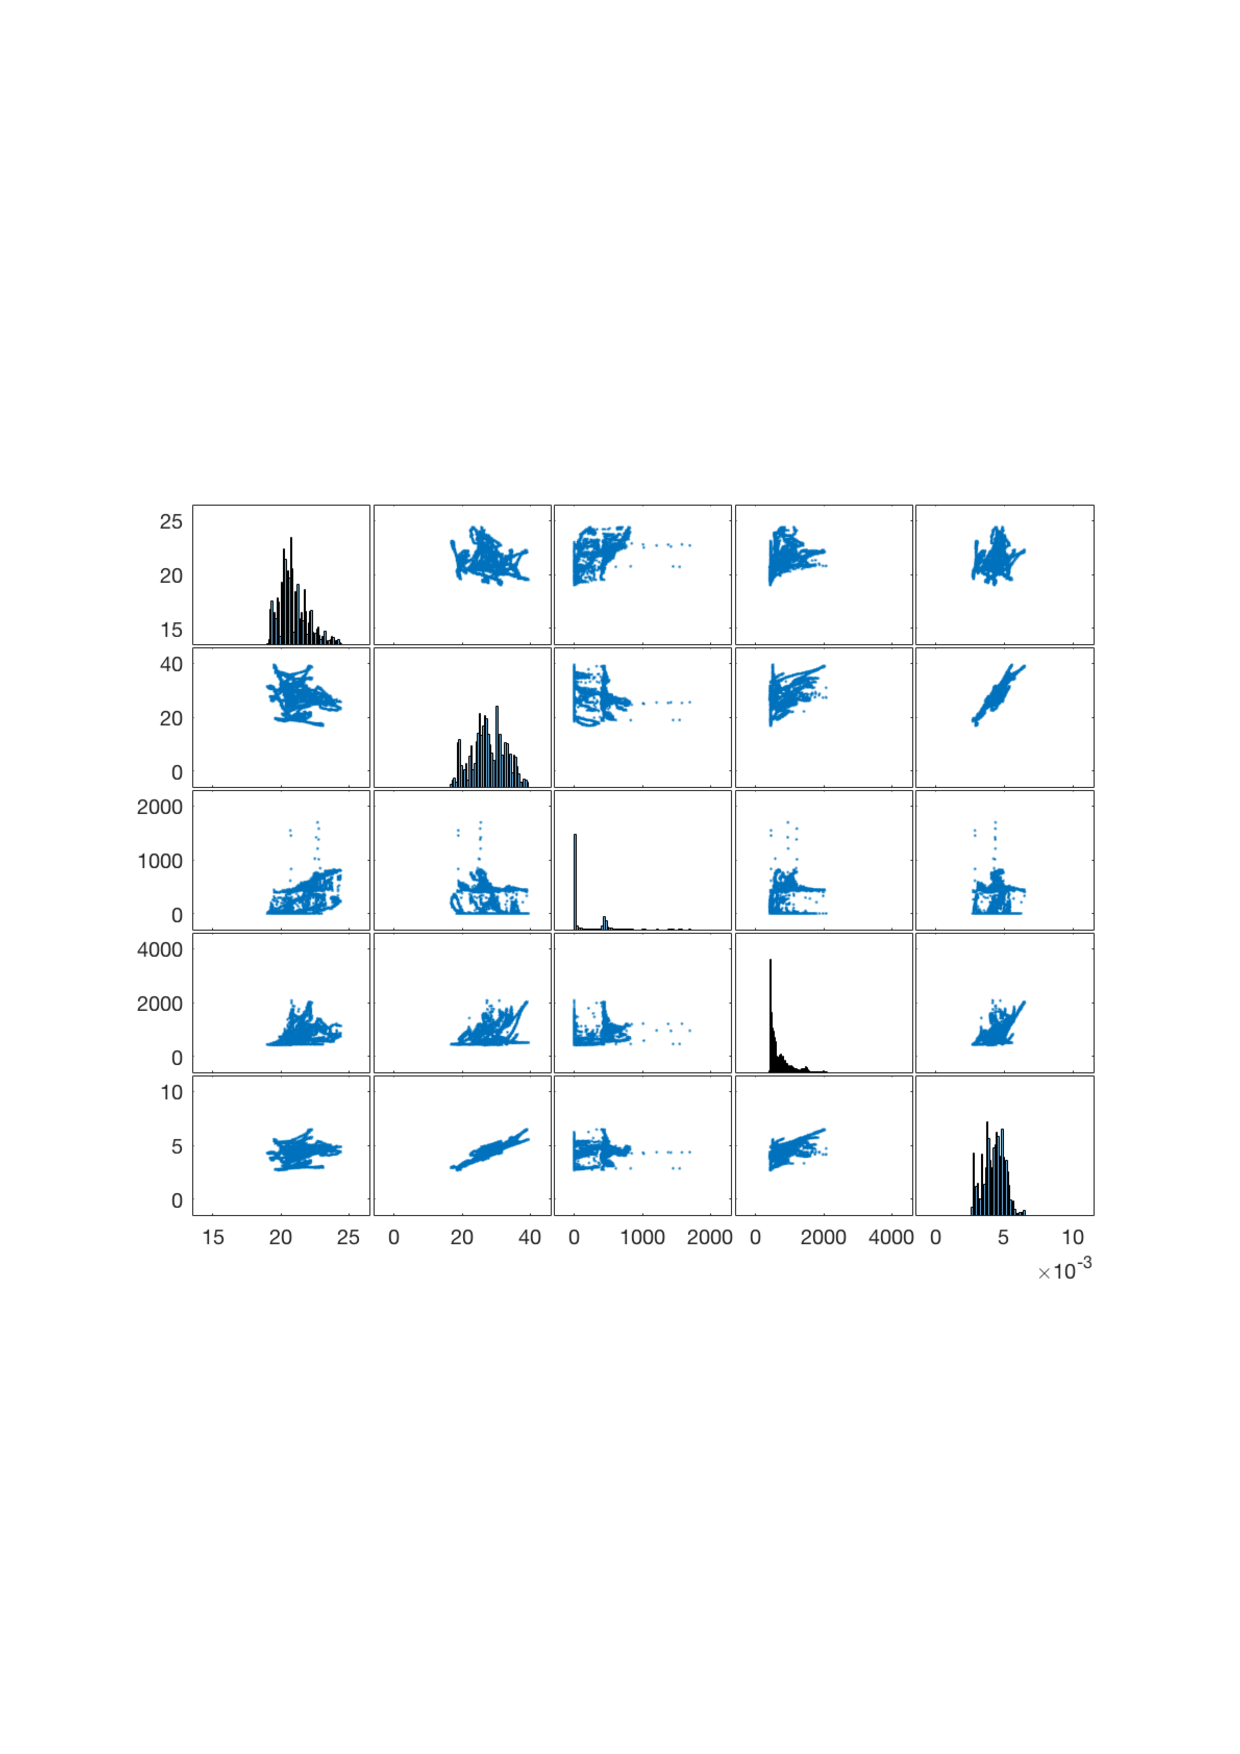
\includegraphics[width=8cm]{plotmatrix1.pdf}
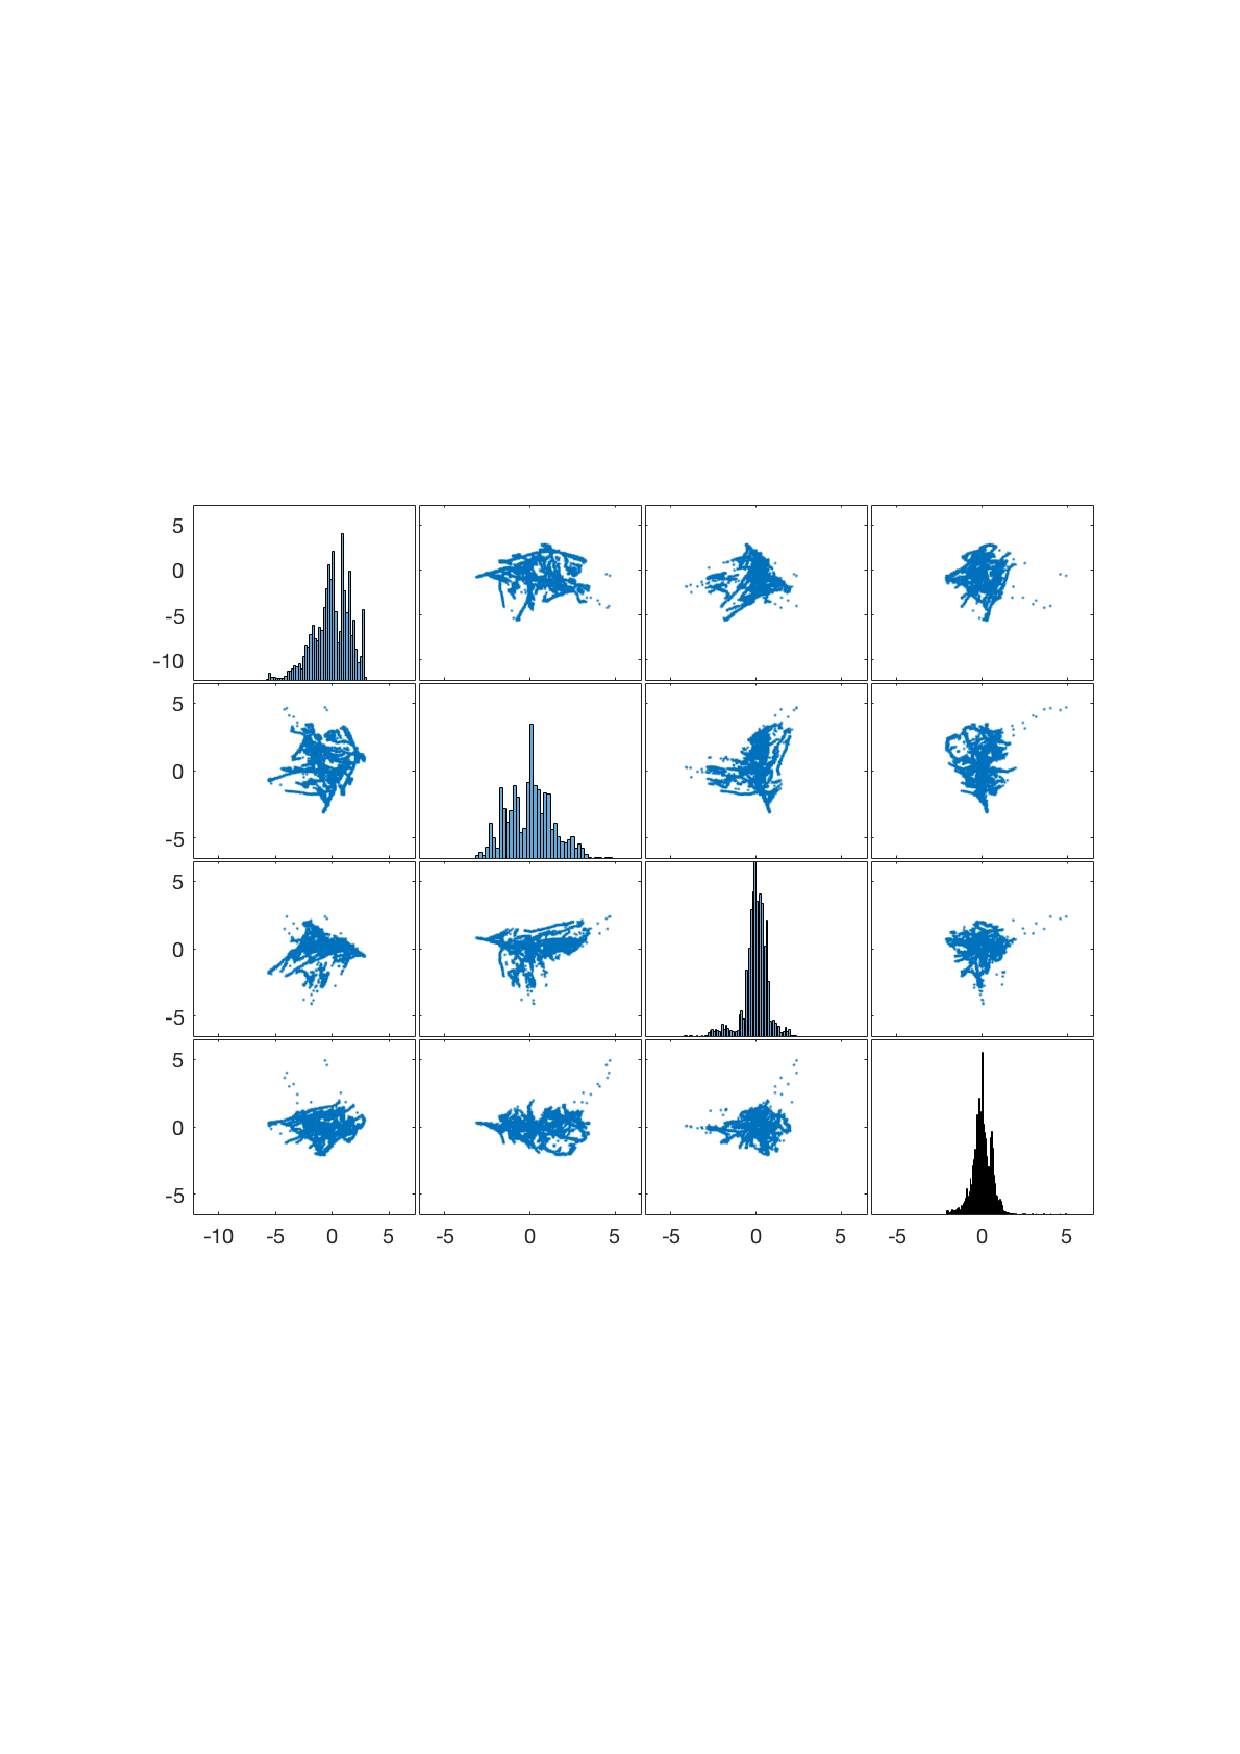
\includegraphics[width=8cm]{plotmatrix2.pdf}
\end{center}
\caption{\label{fig:pca-before-after} Results of $plotmatrix$ of the full dataset before (left) and after (right) PCA.}
\end{figure}

From Figure \ref{fig:pca-before-after}(left), it is clear that some input variables may be skewed, especially \#3 (Light) and \#4 (CO\textsubscript{2}), which may also contain outliers. This makes [0, 1] normalisation with $mapminmax$ potentially unsuitable, as proved by comparison test with unnormalised data, shown in Figure \ref{fig:normalize-testing}.

\begin{figure}[h]
\begin{center}
\fontsize{9}{11}\selectfont
\begin{tabular}{|c|c|c|}
\hline 
Normalisation of Input Dataset & Normalized & Not Normalized \\ \hline
Mean Training MSE & 0.198 & 0.050 \\ \hline \hline 
Mean Validation 1 MSE & 0.138 & 0.064 \\ \hline 
Mean Misclassification 1 (\%) & 16.03 & 2.18 \\ \hline \hline 
Mean Validation 2 MSE & 0.320 & 0.101 \\ \hline 
Mean Misclassification 2 (\%) & 60.53 & 4.58 \\ \hline
\end{tabular}
\end{center}
\caption{\label{fig:normalize-testing} Results from testing the [0, 1] normalisation of training and testing inputs on a [20 1] SOM. (All MSE variances $<0.01$, unnormalised misclassification 2 variance $=5.74$ , rest $<1.00$.)}
\end{figure}

An alternative to normalisation is to first transform input data so that each variable has a mean of 0 and standard deviation of 1, by first applying $mapstd$ then $processpca$ with a maximum fraction of 0.02. This resulted in the removal of one variable -- which makes sense, as variable \#5 Humidity Ratio was calculated from temperature and relative humidity, resulting in a possible correlation. The result of PCA is visualised in Figure \ref{fig:pca-before-after} (right). It is evident that the processed input variables are far less correlated, and could potentially improve the training of SOM.

However, it came to a surprise that this is not the case, after a comparison testing of 10 runs with toolbox defaults on both a [20 1] and a [20 5] network, as shown in Figure \ref{fig:pca-testing}.

\begin{figure}[h]
\begin{center}
\fontsize{9}{11}\selectfont
\begin{tabular}{|c|c|c|}
\hline 
PCA Processing of Input Dataset & After PCA & Before PCA \\ \hline
Mean Training MSE & 0.467 & 0.050 \\ \hline \hline 
Mean Validation 1 MSE & 0.552 & 0.063 \\ \hline 
Mean Misclassification 1 (\%) & 84.65 & 2.17 \\ \hline \hline 
Mean Validation 2 MSE & 0.303 & 0.100 \\ \hline 
Mean Misclassification 2 (\%) & 38.70 & 4.55 \\ \hline
\end{tabular}
\end{center}
\caption{\label{fig:pca-testing} Results from testing the PCA processing of training and testing inputs on a [20 1] SOM. (All MSE variances $<0.01$, unnormalised misclassification 2 variance $=5.50$ , rest $<2.20$.)}
\end{figure}

In order to confirm that the high misclassification rates do not originate from a problem in the assumption of SOM clustering on two ends, and that using a two-dimensional SOM instead will not alleviate the issue, SOM sample hit plots from the training of the [20 1] and another [20 5] SOM are shown in Figure \ref{fig:pca-fail}. It can be observed that in both cases, more than two clusters of the data can be seen for each class, rendering a meaningful binary classification impossible.

\begin{figure}[h]
\begin{center}
Before PCA:\\
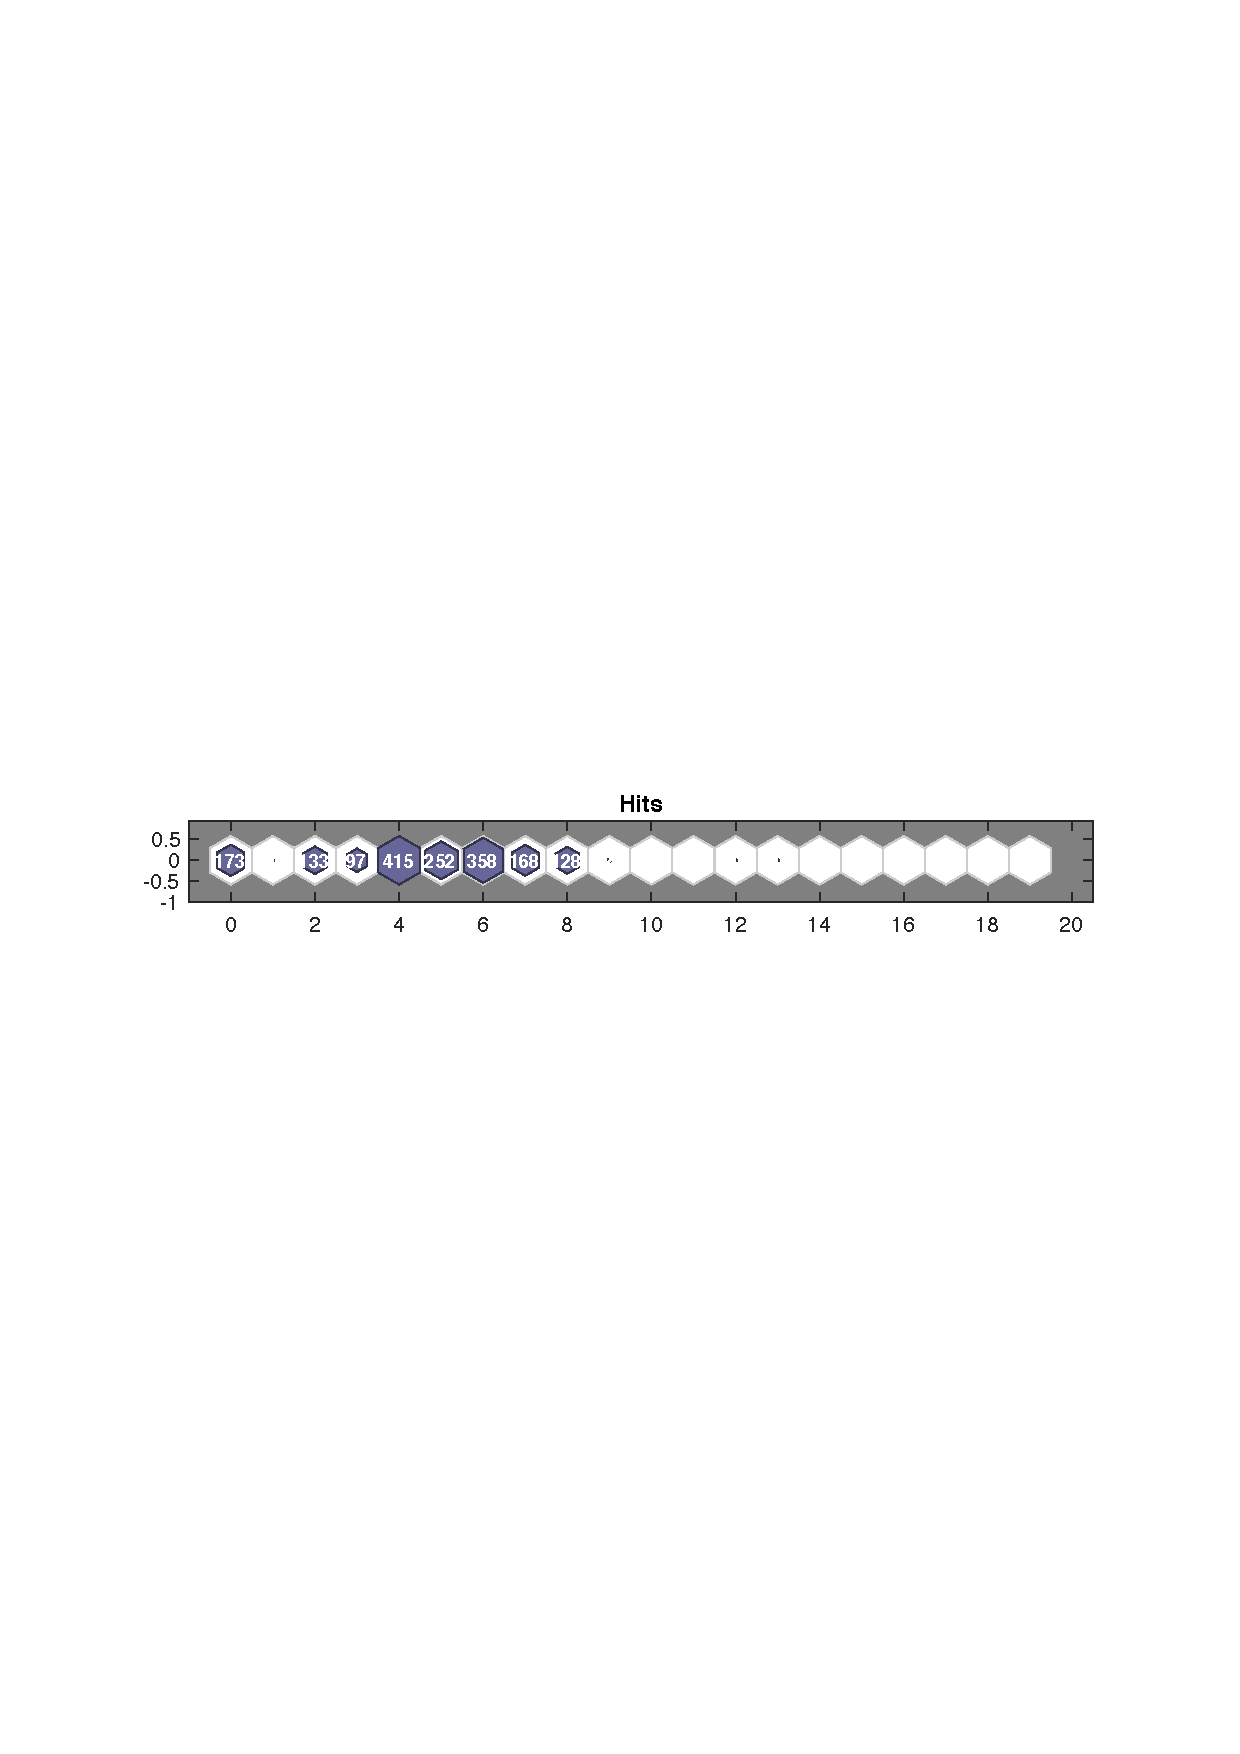
\includegraphics[width=8cm]{nopca-ones.pdf} 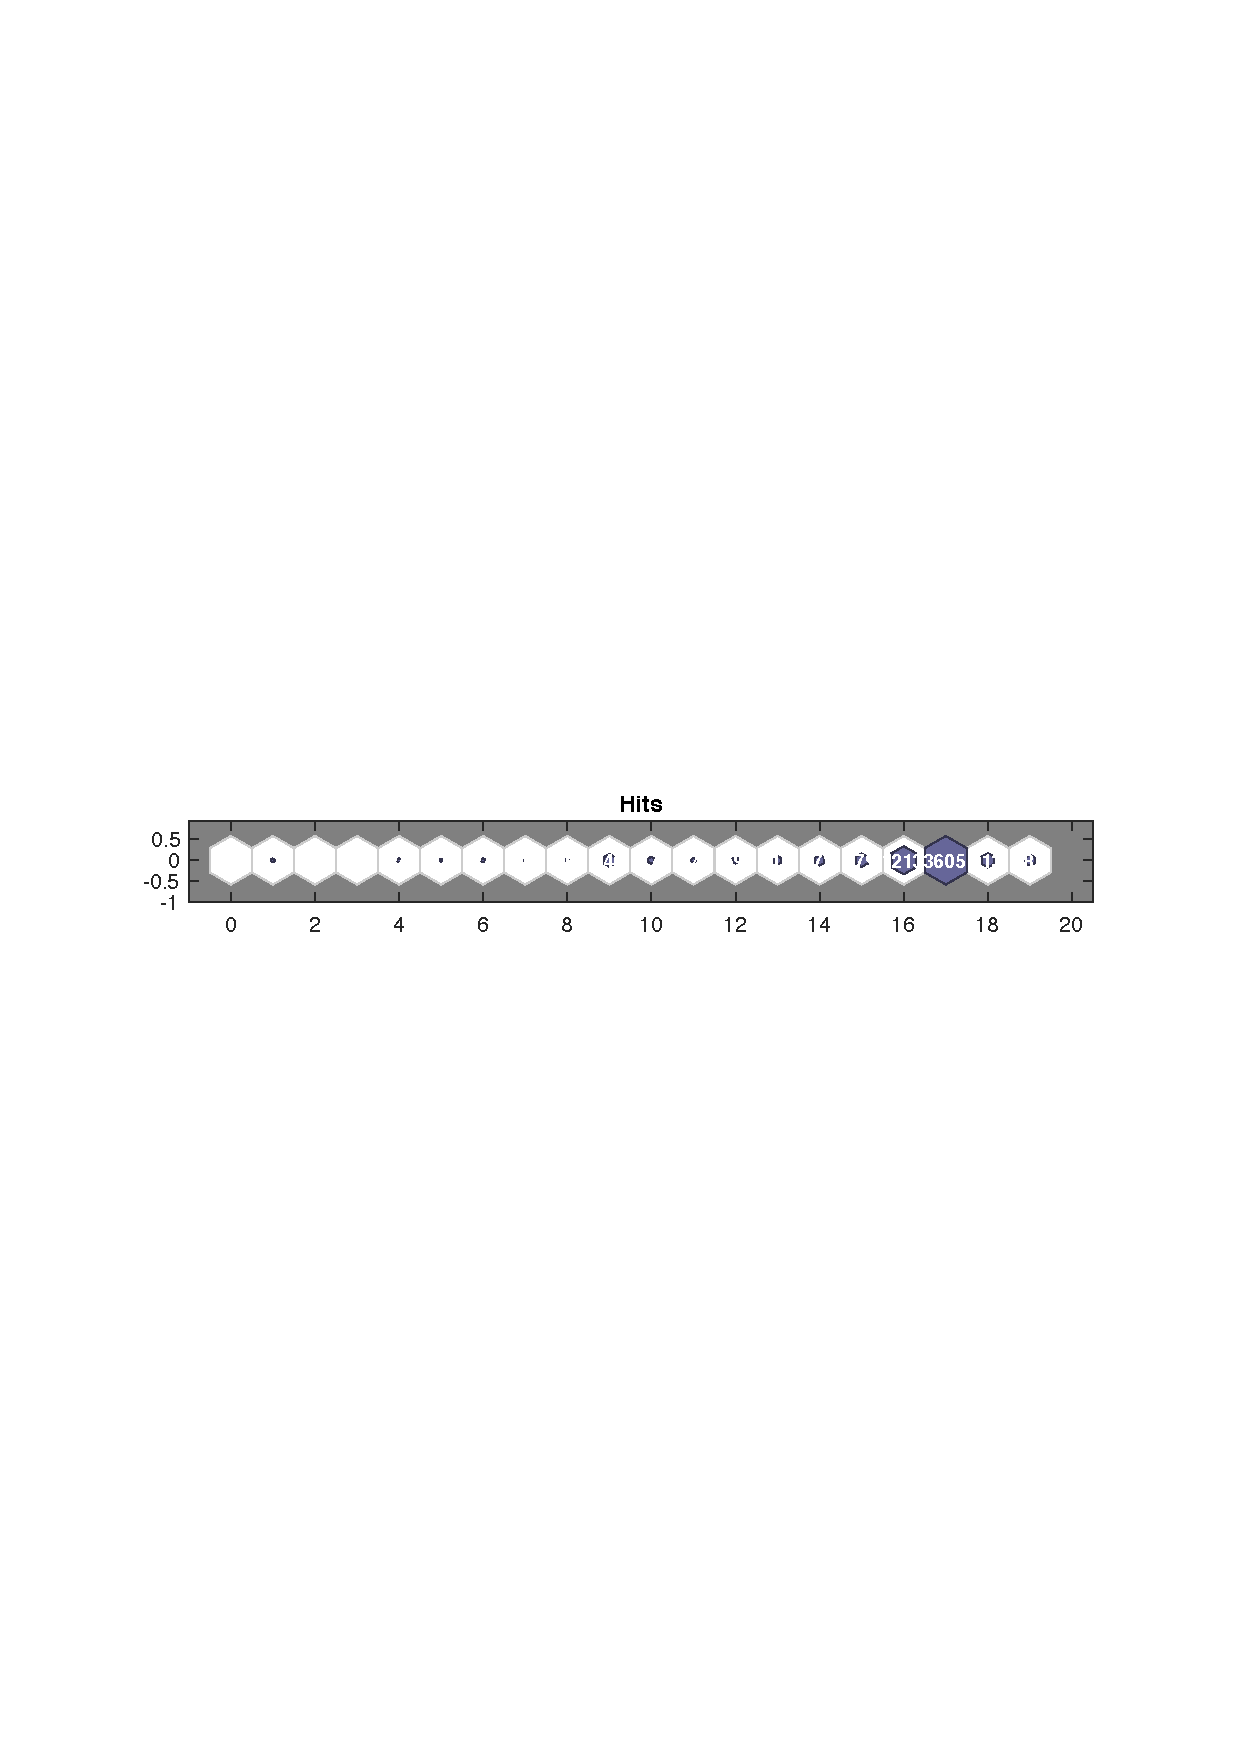
\includegraphics[width=8cm]{nopca-zeros.pdf}\\
After PCA:\\
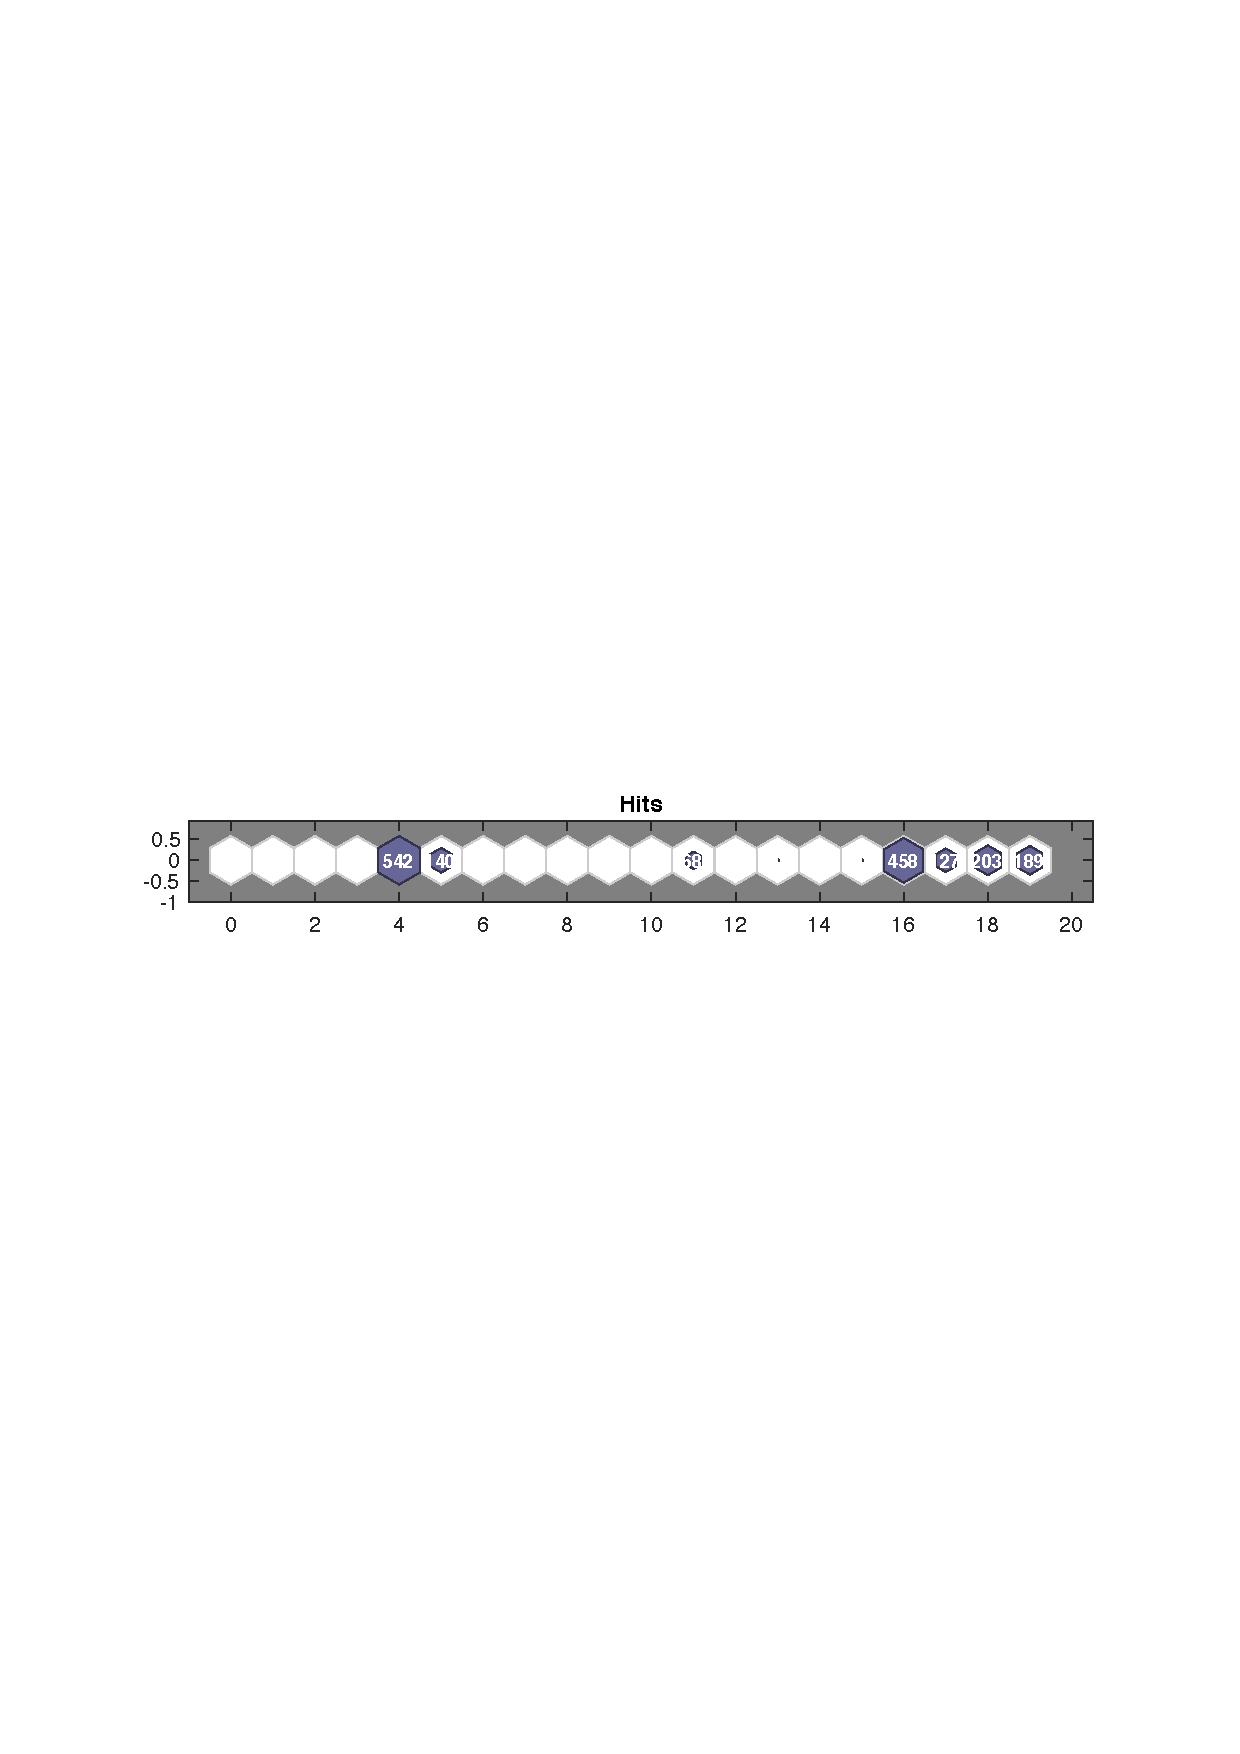
\includegraphics[width=8cm]{pca-fail1-ones.pdf} 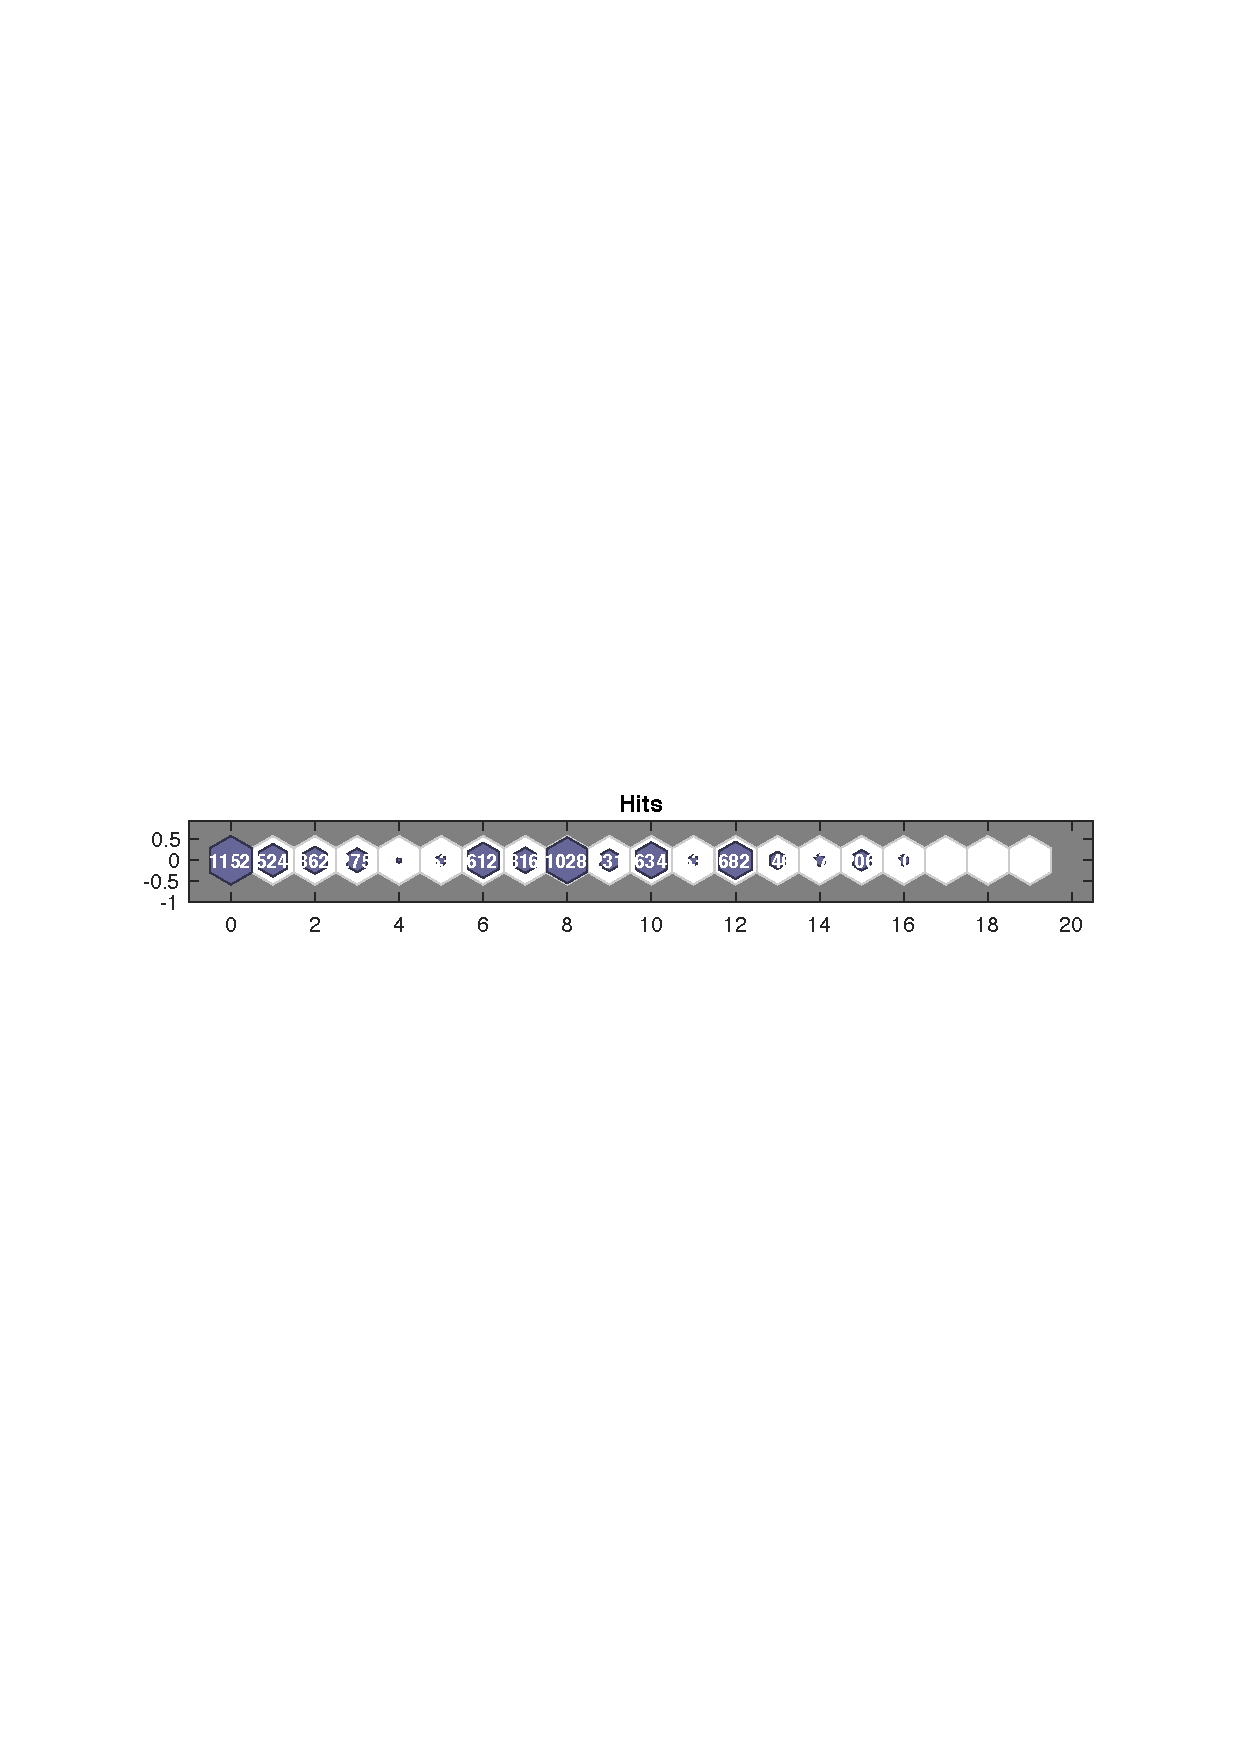
\includegraphics[width=8cm]{pca-fail1-zeros.pdf}
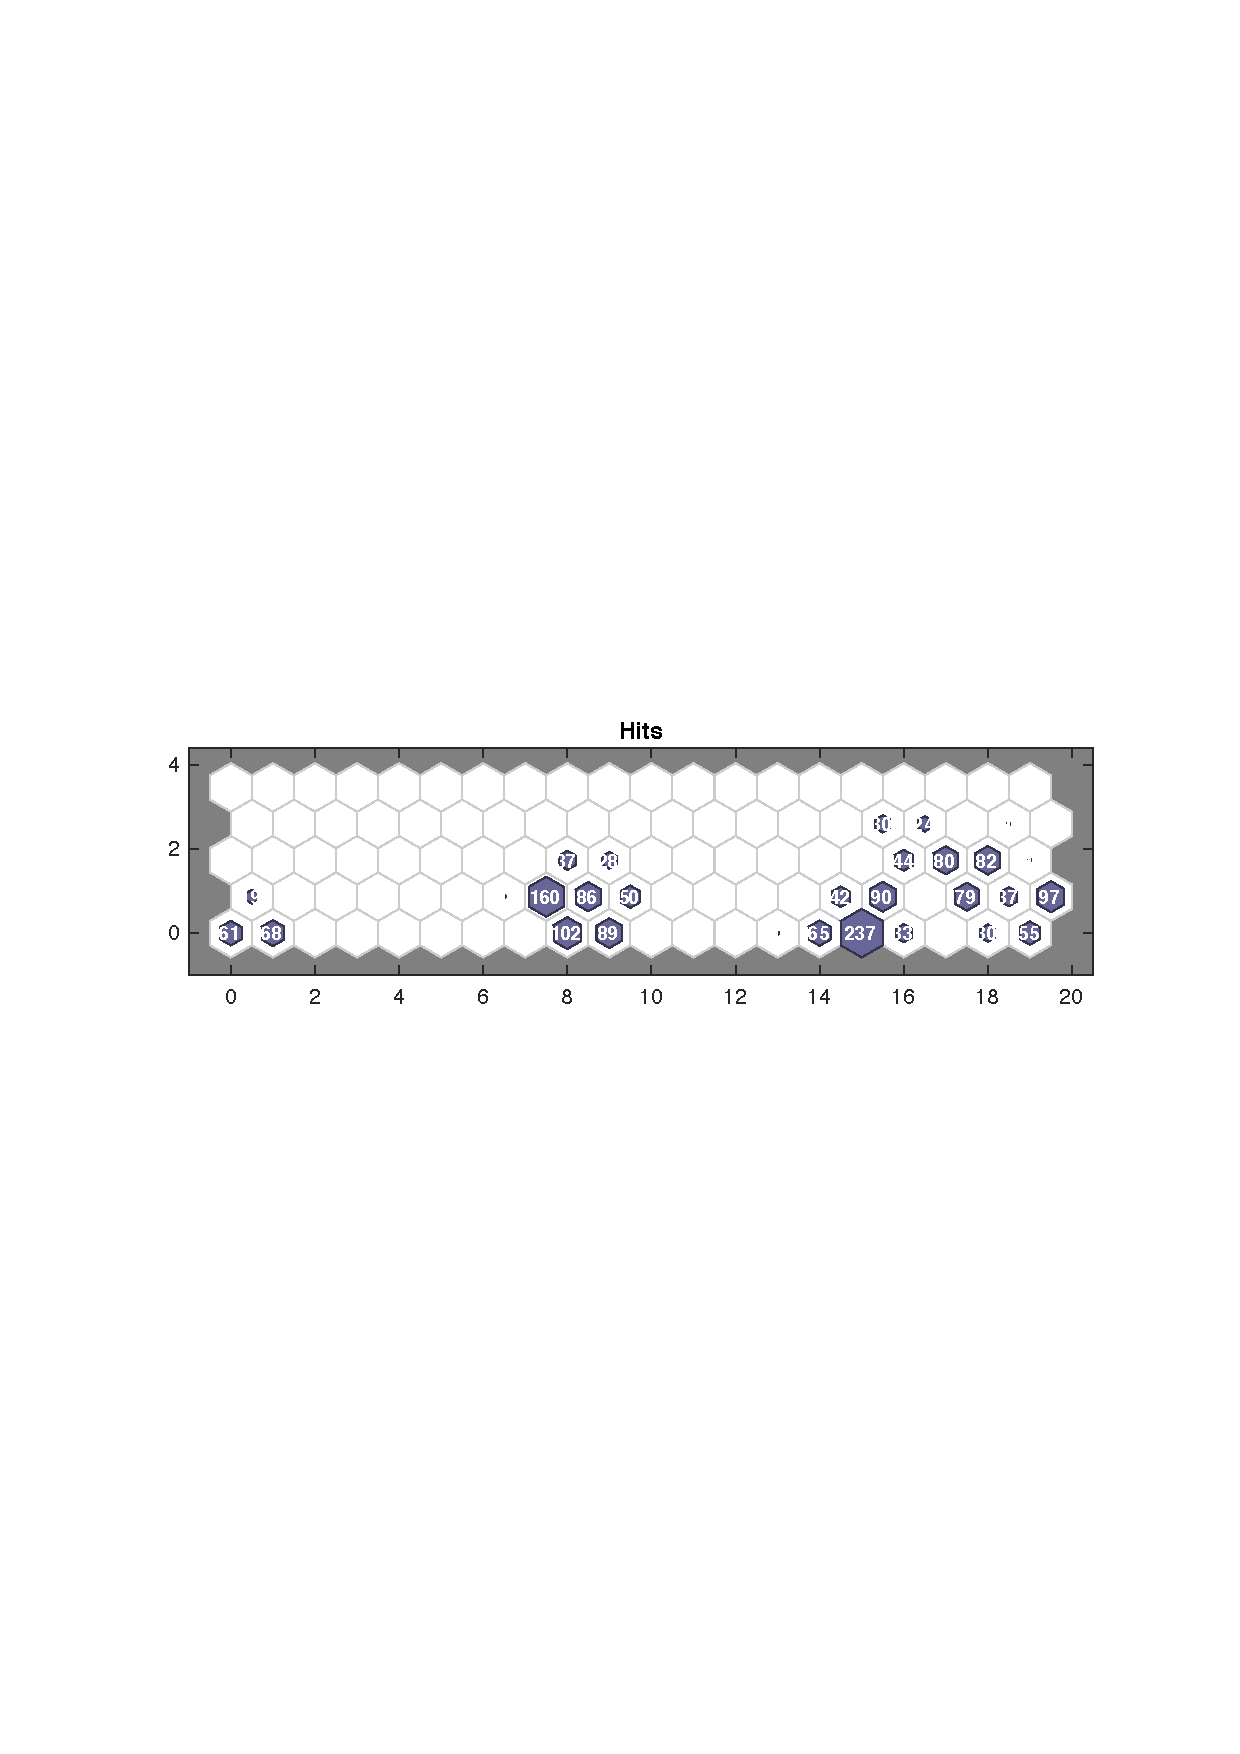
\includegraphics[width=8cm]{pca-fail2-ones.pdf} 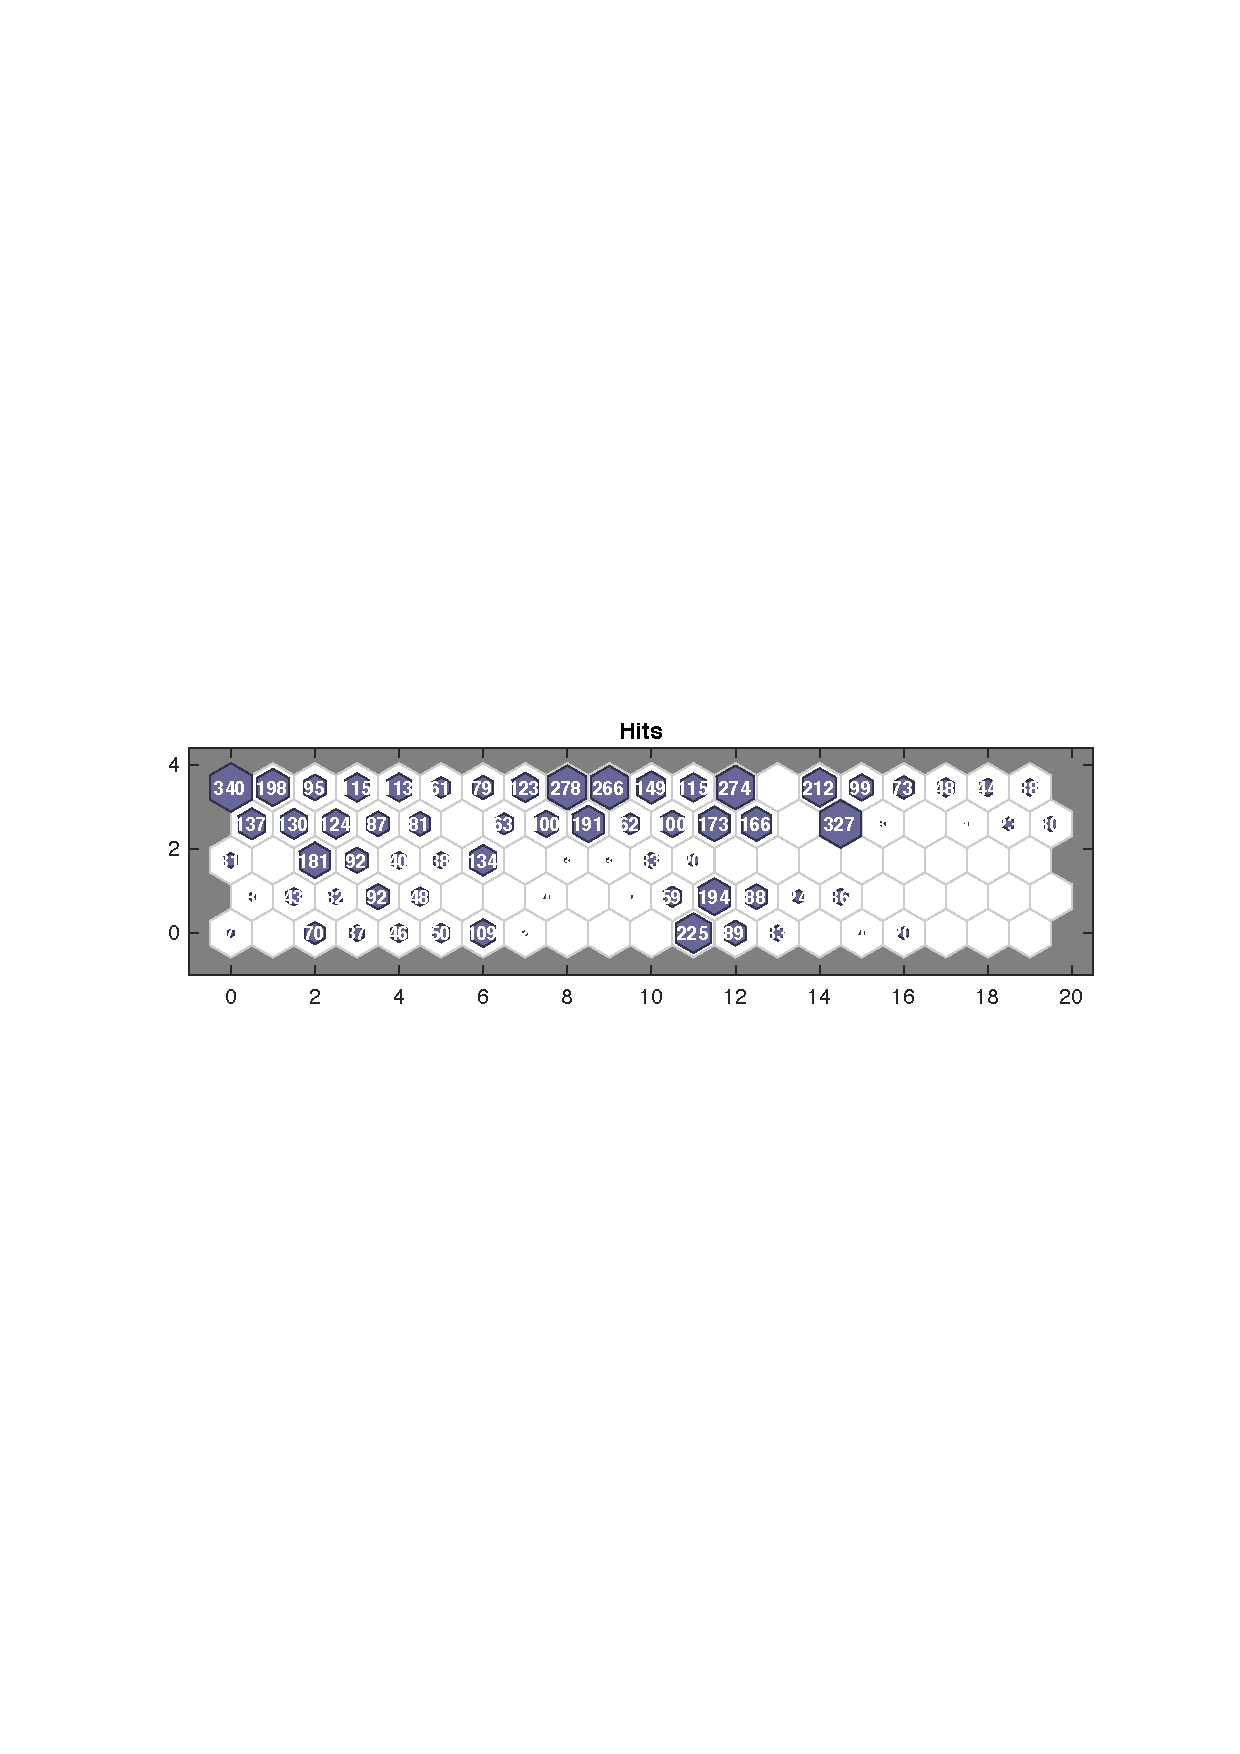
\includegraphics[width=8cm]{pca-fail2-zeros.pdf}
\end{center}
\caption{\label{fig:pca-fail} $plotsomhits$ plots from the training of a [20 1] and a [20 5] SOM on the input data. At the top is the control group (before PCA processing), and at the bottom are SOM plots after PCA (with new SOMs). To the left are occupied cases, and to the right are unoccupied cases.}
\end{figure}

A possible explanation to this interesting observation is that SOM can be considered as a non-linear generalisation of PCA itself \cite[p. 1]{akinduko2012initialization}. Principle component could be used as a method for initialisation of the SOM weight positions, but it is evaluated to perform less well than random initialisation. Therefore, applying PCA on the inputs of SOM may not achieve the same effects as on the inputs of a MLP. 

Considering the fact that the five variables shown in Figure \ref{fig:final-variables} without additional pre-processing already performs very well (single-digit misclassification percentages) as the baseline for the few comparisons performed in this section, it was decided that \textbf{the five input variables will be used as is for the SOM without further processing}.

\subsection{Description of the SOM architecture}

The self-organising map (SOM) represents a unique feedforward architecture. The architecture consists of a mesh of connected neurons, each selectively tuned for specific features of the input data during the training process \cite[Sec. 9.1]{haykin2008}. The mesh of neurons are topologically ordered \cite[p. 11]{som-lecture}, which implies that a specific point on the map formed by these neurons maps to a specific set of characteristics seen in a certain set of input data. This feature allows SOM to be used to solve simple classification problems such as this one, in addition to its very useful purposes in projecting high-dimensionally data nonlinearly to achieve purposes such as visualisation. Two models of this mapping process exist: the Willshaw-von der Malsburg's model and the Kohonen model \cite[Sec. 9.2]{haykin2008}, and the MATLAB toolbox uses the Kohonen model \cite{som-matlab}, to be described in more detail in Section \ref{subsec:training}.

The SOM is implemented with the $selforgmap$/$newsom$ and associated methods in the MATLAB Neural Network Toolbox \cite{kohonen2014matlab}. For all of the preliminary testings in the previous sections, the default parameters for the network are used: 100 epochs in each phase of the training (phases to be covered in \ref{subsec:training}), initial neighbourhood size of 3 (to be later reduced), arranged in a hexagonal topology with linked distance as the distance function. In addition, the legacy $newsom$ method also allows the creation of same SOMs with adjustable learning rates, at this time they are set to defaults. Later in Section \ref{subsec:training}, changes to some of these parameters will be explored.

The architecture of the SOM is relatively simple to implement: an input layer of a set number of neurons connects to a single layer of map neurons (nodes) topographically arranged in a mesh, the dimensions of which are defined by the network configuration. This forms a feedforward structure \cite[p. 429]{haykin2008}. Each map neuron has a set of weights in its connections with neurons on the input layer, which affects the length of the connection, resulting in the surface of the mesh to ``bend'' as the weights change. At initialisation, various methods can be used to initialise these weights. The toolbox default creates linearly separated sets of weight, and places the same number of neurons on the input layer as there are input variables, as shown in Figure \ref{fig:som-init}.

Lateral connections are also to be created between neighbouring neurons based on the topology. Their positions are useful to the distance function such as linked distance (which means distances are immutable in this case, as $linkdist$ counts by neuron only), as discussed above. In the case of the one-dimensional mesh used in this report, the lateral connections are much simpler due to the simplified structure (at most two connections per neuron), as shown in Figure \ref{fig:som-init} (left). A visual illustration of another SOM with dimensions [5 2] is shown in Figure \ref{fig:som-visual}.

\begin{figure}[h]
\begin{center}
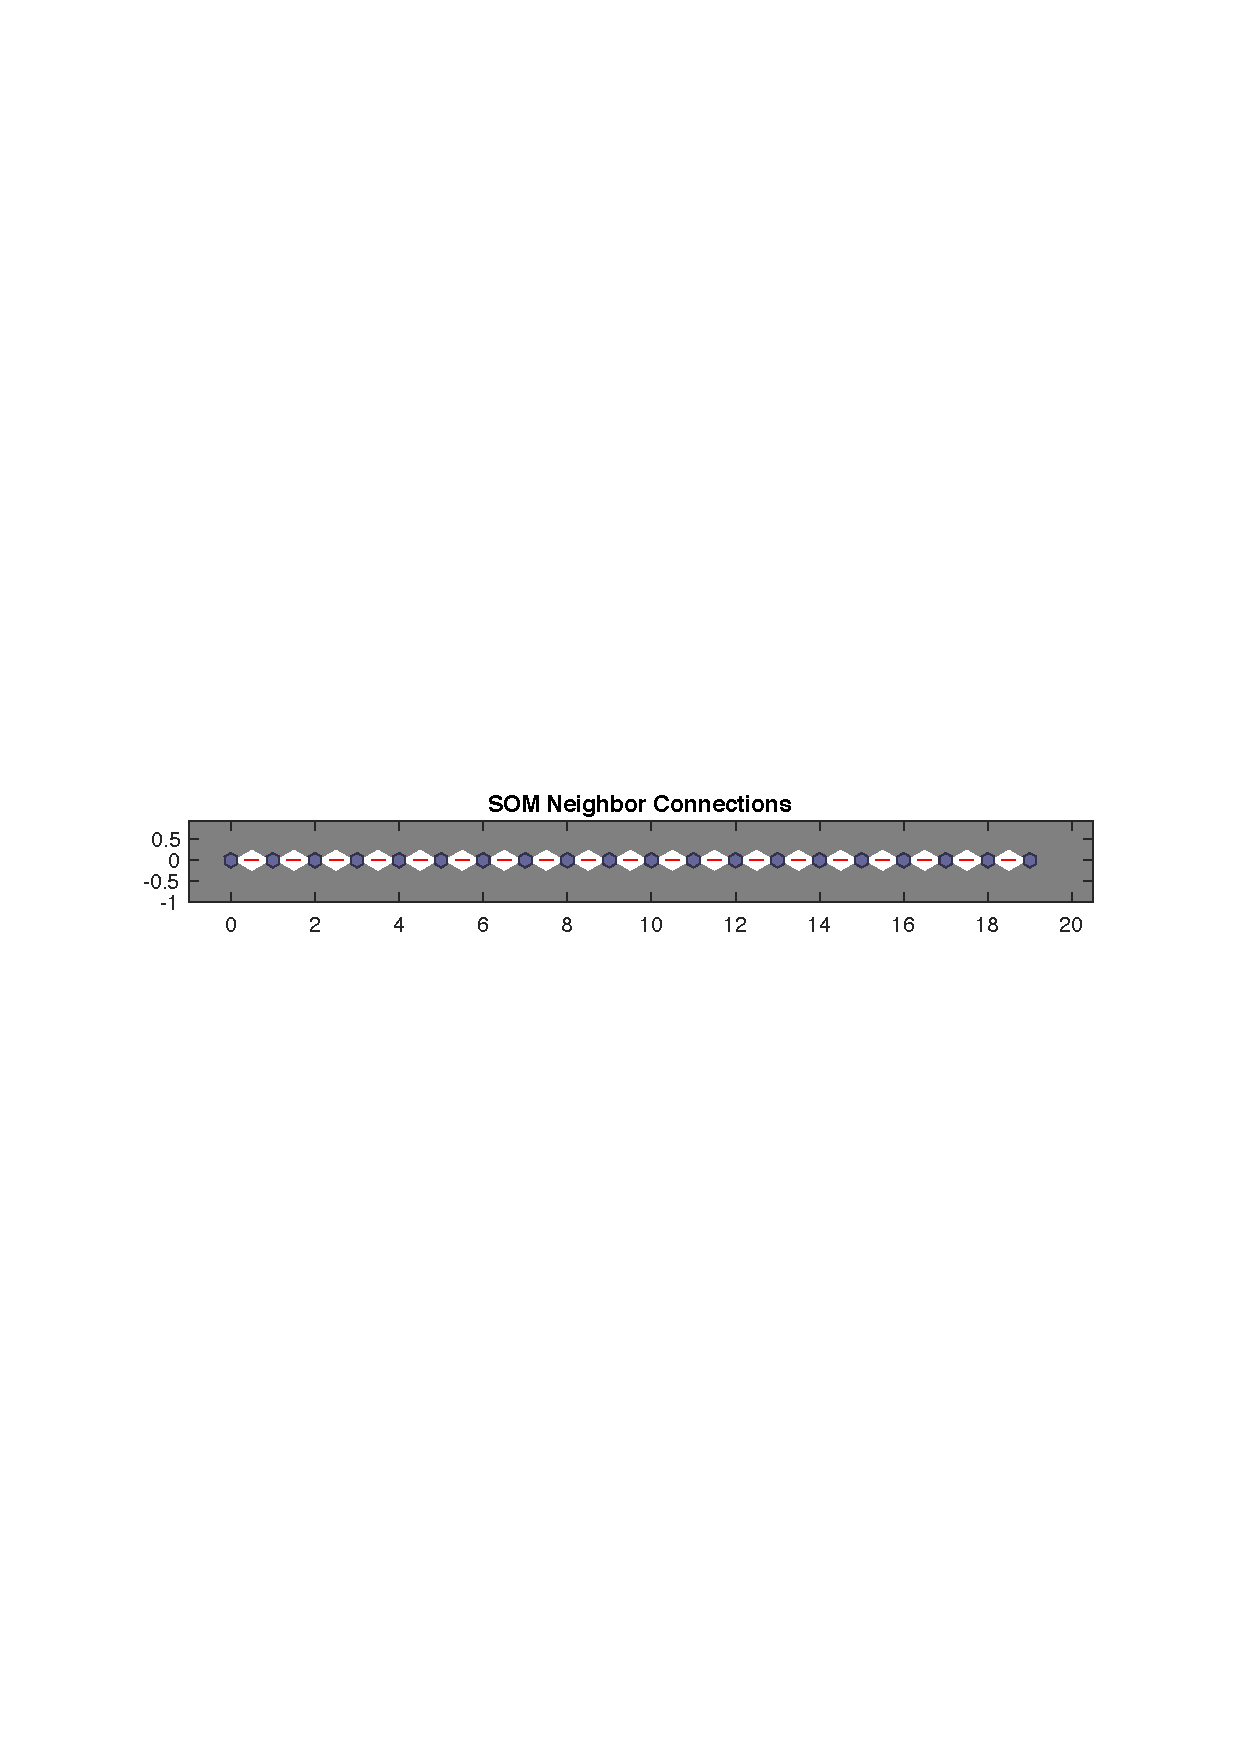
\includegraphics[width=8cm]{somnc.pdf} 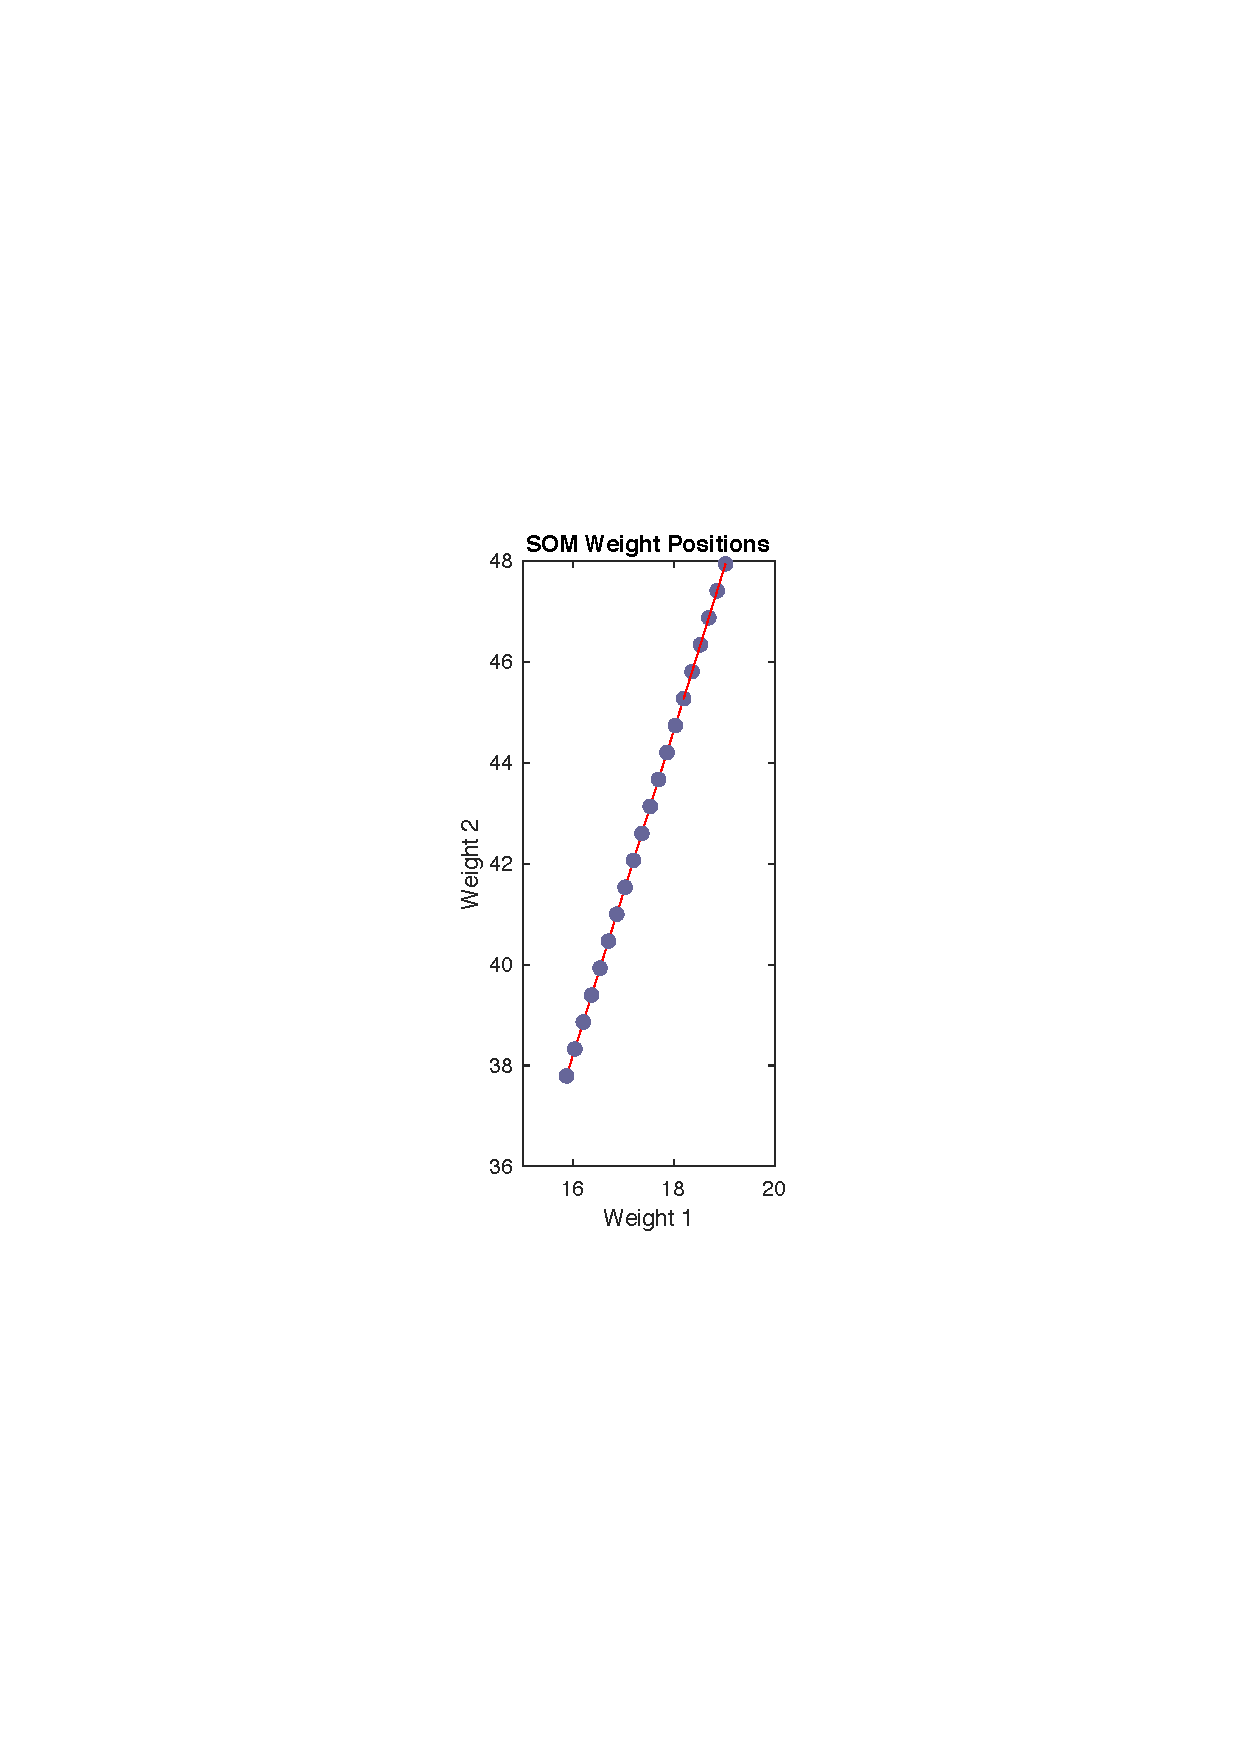
\includegraphics[width=2.07cm]{sompos.pdf} 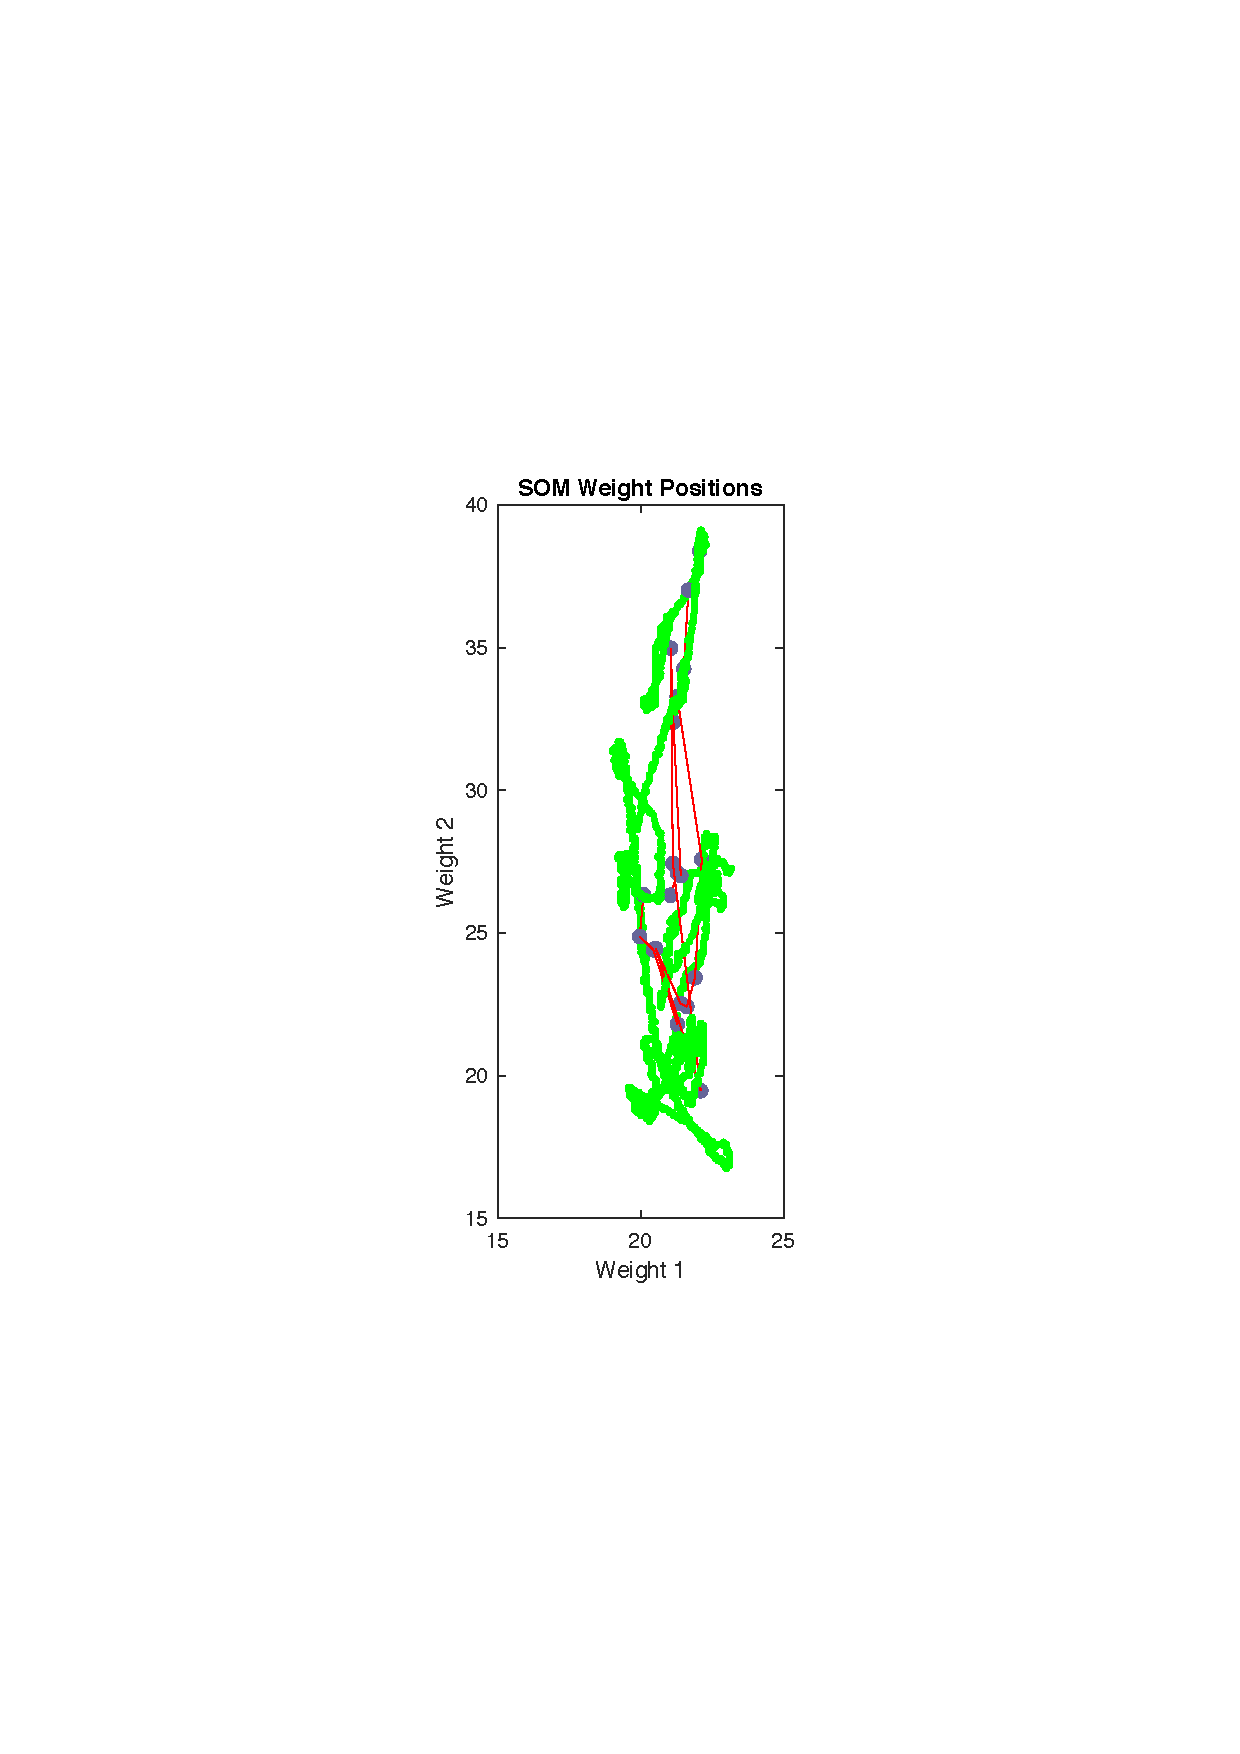
\includegraphics[width=2cm]{sompos-aftertraining.pdf}
\end{center}
\caption{\label{fig:som-init} The initial neighbour connections and weight positions (first two of five) of the SOM created by the toolbox (left), as well as the weight positions of the same inputs after training (right).}
\end{figure}

\begin{figure}[h]
\begin{center}
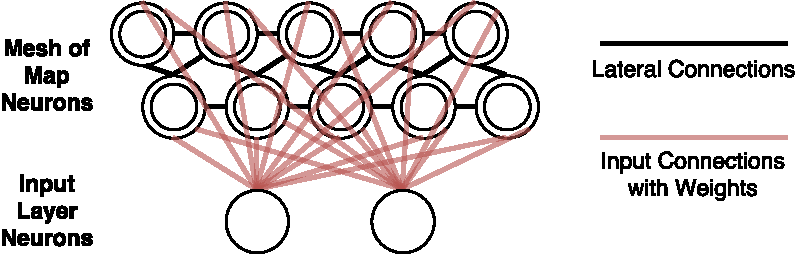
\includegraphics[width=12cm]{som-visual.pdf} 
\end{center}
\caption{\label{fig:som-visual} Visual illustration of a SOM with dimensions [5 2] and two input neurons (possibly connecting two input variables). The mesh is arranged in $hextop$ grid.}
\end{figure}

\subsection{Training of the SOM architecture} \label{subsec:training}
 
Unlike MLP, a Kohonen SOM has a defined way of training, implemented in the toolbox as $trainbu$. The training is divided into two, usually equal-length phases: the ordering phase and the convergence phase \cite[p. 23]{som-lecture}. The purpose of the training process is to expose all neurons to a sufficient number of different input patterns with different corresponding active spots on the map \cite[p. 429]{haykin2008}, adjusting the input weights and therefore allowing the network to produce distinct responses for different classes of input patterns. Haykin \cite[p. 435]{haykin2008} recommends 1000 steps for each phase of the training. The MATLAB toolbox default is 100 for each phase \cite{som-matlab}, which produced a general classification accuracy of $>95$\% in cursory and data testing as shown in the previous sections.

The two training phases are procedurally identical, but different in the values of learning rate ($\eta$) and neighbourhood size ($\sigma$), both of which smaller in the convergency phase than the ordering phase, as the ordering phases is responsible for main topological ordering, while the convergency phase is used for fine tuning between neighbouring neurons \cite[p. 23]{som-lecture}. The starting learning rates are $\eta=0.9$ and $\eta=0.02$, and the start neighbourhood sizes are the entire mesh's radius and $\sigma=1$ respectively for the ordering and convergence phases \cite{newsom-matlab}. These values are close to the recommended start values\cite[p. 23]{som-lecture}. During each phase, exponential functions gradually reduces these parameters, as described below.

Each step during either phase is a three-stage process: competition, cooperation and adaptation \cite[pp. 429-430]{haykin2008}. The first stage determines the most excited (winning) neuron, which is used to determine a neighbourhood in the second stage, through a neighbourhood function $h$. Neurons in the neighbourhood selected then have their weights adjusted to be closer to the most excited neuron in the last stage. This process repeats until a defined number of steps are completed for each phase.

In the competition phase, with an input space of $m$ variables and the particular input $x$, the selection of the most excited neuron $i(x)$ on a mesh of neurons (each neuron $j$ with a weight vector $w_j$) is with the following algorithm \cite[p. 430]{haykin2008}:
\begin{equation}
i(x) = arg \min_{j}\|x  - w_{j}\| \ \text{, where}\ x = [x_1, x_2, ..., x_m]^T \ \text{and} \ w_j = [w_{j1}, w_{j2}, ..., w_{jm}]^T
\end{equation}

In the cooperation phase, owing to the observation that neurons closer to the winning neuron assimilate more towards the winning neuron than the neurons further away, the neighbourhood function $h$ determines the scale of activation, based on the set neighbourhood size $\sigma$, and the distance $d_{ji}$ from the winning neuron determined by a distance function, such as linked distance ($linkdist$) \cite[p. 431]{haykin2008}:
\begin{equation}
h_{ji} = exp(-\frac{d^2_{ij}}{2\sigma^2}) \ \text{for lateral distance between the winning neuron $i$ and neighbouring neuron $j$}
\end{equation}

And finally, in the adaptation phase, neurons in the neighbourhood of the winning neuron will assimilate towards the winning neuron. The new weight $w_j(n+1)$ of neuron $j$ is updated at the $n+1$ step as followed \cite[p. 21]{som-lecture}:
\begin{equation}
w_j(n+1) = w_j(n) + \eta h_{ji}(n)(x-w_j(n))
\end{equation}

To achieve a gradual process of weight adjustment, the learning rate $\eta$ and the neighbourhood size $\sigma$ are generally exponentially reduced over time \cite[pp. 21-22]{som-lecture}:
\begin{equation}
\eta (n) = \eta_0 exp(-\frac{n}{\iota}) \;\;\;\;\;\;\;  \sigma (n) = \sigma_0 exp(-\frac{n}{\iota'})
\end{equation}

While there is no choice of training algorithms, it is possible to alter the number of steps in each phrase of training, as well as the initial learning rates $\eta$ and neighbourhood sizes $\sigma$ to observe their effects on the performance of the trained SOM. Based on the recommendations from the module \cite{som-lecture} and Haykin \cite{haykin2008}, several different combinations of training steps, learning rates and neighbourhood sizes are chosen, each tested ten times on a fresh [20 1] SOM. 

First, to test the influence of number of steps in each phase, a few training configurations are tested with the default learning rates and neighbourhood sizes, as shown in Figure \ref{fig:steps-testing}.

\begin{figure}[h]
\begin{center}
\fontsize{9}{11}\selectfont
\begin{tabular}{|c|c|c|c|c|c|c|c|}
\hline 
Number of Steps in Each Phase & Type & 100 & 250 & 500 & 750 & 1000 & 2000\\ \hline
\multirow{2}{*}{Training MSE} & Mean & 0.050 & 0.068 & \\ \hline 
& Variance & \<0.01 & \<0.01 &  \\ \hline
\multirow{2}{*}{Validation 1 MSE} & Mean & 0.064 & 0.094 & \\ \hline 
& Variance & \<0.01 & \<0.01 & \\ \hline
\multirow{2}{*}{Misclassification 1} (\%) & Mean & 2.18 & 3.45 & \\ \hline 
& Variance & \<0.01 & 0.283 &  \\ \hline
\multirow{2}{*}{Validation 2 MSE & Mean & 0.101 & 0.127 & \\ \hline 
& Variance & \<0.01 & \<0.01 & \\ \hline
\multirow{2}{*}{Misclassification 2 (\%) & Mean & 4.54 & 4.96 \\ \hline
& Variance & 5.38 & 7.02 & \\ \hline
\end{tabular}
\end{center}
\caption{\label{fig:steps-testing} Results from varying the number of steps in each phase of training on a [20 1] SOM. The total number of training epochs is twice this number.}
\end{figure}

\subsection{Evaluation of the trained SOM}

Before starting the evaluation of the trained SOM, it is necessary to first discuss in more detail how the actual misclassification rates (``Misclassification \%'') are calculated. As described at the start of Section \ref{subsec:preprocessing}, an assumption was made that the one-dimensional SOM will cluster the two classes of inputs at the two ends of the map. During the course of this report, extensive observations on $plotsomhits$ have always showed that this is the case on one-dimensional SOMs without normalisation or PCA conducted on the input data. 

It was also observed that the positions of the two clusters have always been opposite to the ordering of the output vector (occupied/`1' inputs cluster on the left, unoccupied/`0' inputs cluster on the right. This is however, a projection of data in higher dimensions, and maybe arbitrary \cite[p. 10]{som-app-lecture}. While it appears that the toolbox implementation always projects the output data in this orientation, this is not a defined feature of the network.

Therefore, it was possible to infer the class of an input, based on its position in the output vector from applying the SOM on that input. However, as the assumptions made may be implementation specific (i.e. to the MATLAB toolbox), some manual observations on the results of other implementations may be required before these assumptions can be carried over.

\bibliographystyle{IEEEtran}
\small{\bibliography{report}}
\end{document}  